\documentclass[conference]{IEEEtran}
\IEEEoverridecommandlockouts
% The preceding line is only needed to identify funding in the first footnote. If that is unneeded, please comment it out.
%Template version as of 6/27/2024

\usepackage{cite}
\usepackage{amsmath,amssymb,amsfonts}
\usepackage{graphicx}
\usepackage{textcomp}
\usepackage{xcolor}
\usepackage{subcaption}
\usepackage{booktabs}
\usepackage{tabularx}
\usepackage{algorithm}
\usepackage{algpseudocode}


\def\BibTeX{{\rm B\kern-.05em{\sc i\kern-.025em b}\kern-.08em
    T\kern-.1667em\lower.7ex\hbox{E}\kern-.125emX}}
\begin{document}

\title{A Two-Phase Dataflow Algorithm for SpMV on the Cerebras Wafer-Scale Engine\\

    \thanks{Identify applicable funding agency here. If none, delete this.}
}

\author{\IEEEauthorblockN{Maya Taylor, Luke Olson}
    \IEEEauthorblockA{\textit{Department of Computer Science} \\
        \textit{University of Illinois at Urbana-Champaign}\\
        Champaign, IL USA \\
        mayat4@illinois.edu, lukeo@illinois.edu}}


\maketitle

\begin{abstract}
    Sparse linear algebra kernels are foundational to scientific computing, but also notoriously difficult to accelerate. Particular challenges arise due to their irregular memory access and load imbalance. We investigate these challenges on a spatial dataflow architecture: the Cerebras Wafer-Scale Engine (WSE). Designed for dense neural network workloads, this architecture promises extremely low latency memory access but requires the right algorithm and data placement, presenting a difficult design problem for sparse workloads.

    The sparse matrix-vector product (SpMV) is a simple but valuable first case study on the WSE.
    We present the first algorithm for SpMV on the WSE and a companion communication model.
    We evaluate both across various matrix sizes and structures, demonstrating the accuracy and utility of the communication model and discussing its shortcomings.
    We also compare the WSE SpMV implementation to a CuSparse equivalent for context to more conventional implementation performance.
    This work provides insight into the utility of spatial dataflow architectures for general sparse workloads and
    informs the most important directions for future work.
\end{abstract}

\begin{IEEEkeywords}

\end{IEEEkeywords}

\section{Introduction}
\begin{enumerate}
    \item The broad goal: explore general unstructured sparse operations on dataflow.
    \item We approach this problem through 1D collectives (easy to model and understand) and spmv (simple but performance very connected to sparsity structure, and easy to map to the 1D collectives)
\end{enumerate}
The big ideas:
\begin{enumerate}
    \item what is the performance model and what are its shortcomings
    \item  is the performance model accurate
    \item  how do we make decisions about layout and resources for optimal performance?
    \item lower and upper performance bounds?
    \item is the spmv performant? compare to GPU
\end{enumerate}

\section{Background}
\subsection{WSE Architecture}
\subsection{Tungsten and Paint}
\subsection{Matrix-Free Approaches for SpMV on Cerebras}
\subsection{Related Work }
Spmv on other architectures
\section{1D Collectives}
\begin{enumerate}
    \item Luczynski et al presents the chain reduce and multicast broadcast that we use.
    \item They also present performance model
    \item We implement the same things in Tungsten + Paint and an updated performance model.
    \item The updates: 2P factor for broadcast, reticle boundary overhead.
\end{enumerate}

\subsection{Pairwise Pingpong}
\begin{enumerate}
    \item Pairwise pingpong benchmark highlights the immediate neighbor communication latency.
    \item Also highlights the reticle boundary crossing.
    \item Experiments show that ramp latency $T_r = 5$
    \item Experiments: within reticle pingpong = 14 cycles. Across reticle = 14 + 18.
    \item Takeaway: PE to PE latency = 2, across reticle 9 additional cycles
\end{enumerate}

\subsection{Broadcast}
\begin{enumerate}
    \item We increase the latency term from $P$ in Luczynski et al to $2P$.
    \item This model is more accurate and also correspons with the 2 cycle PE to PE latency above.
    \item Also add a reticle overhead term, based on how many reticles are crossed.
\end{enumerate}

\subsection{Reduction}
\begin{enumerate}
    \item The model stays the same except $T_r$ and reticle term
    \item Matches super well!
\end{enumerate}

\subsection{Model Performance}

\begin{figure}[htbp]
    \centering
    \begin{subfigure}{0.48\textwidth}
        \centering
        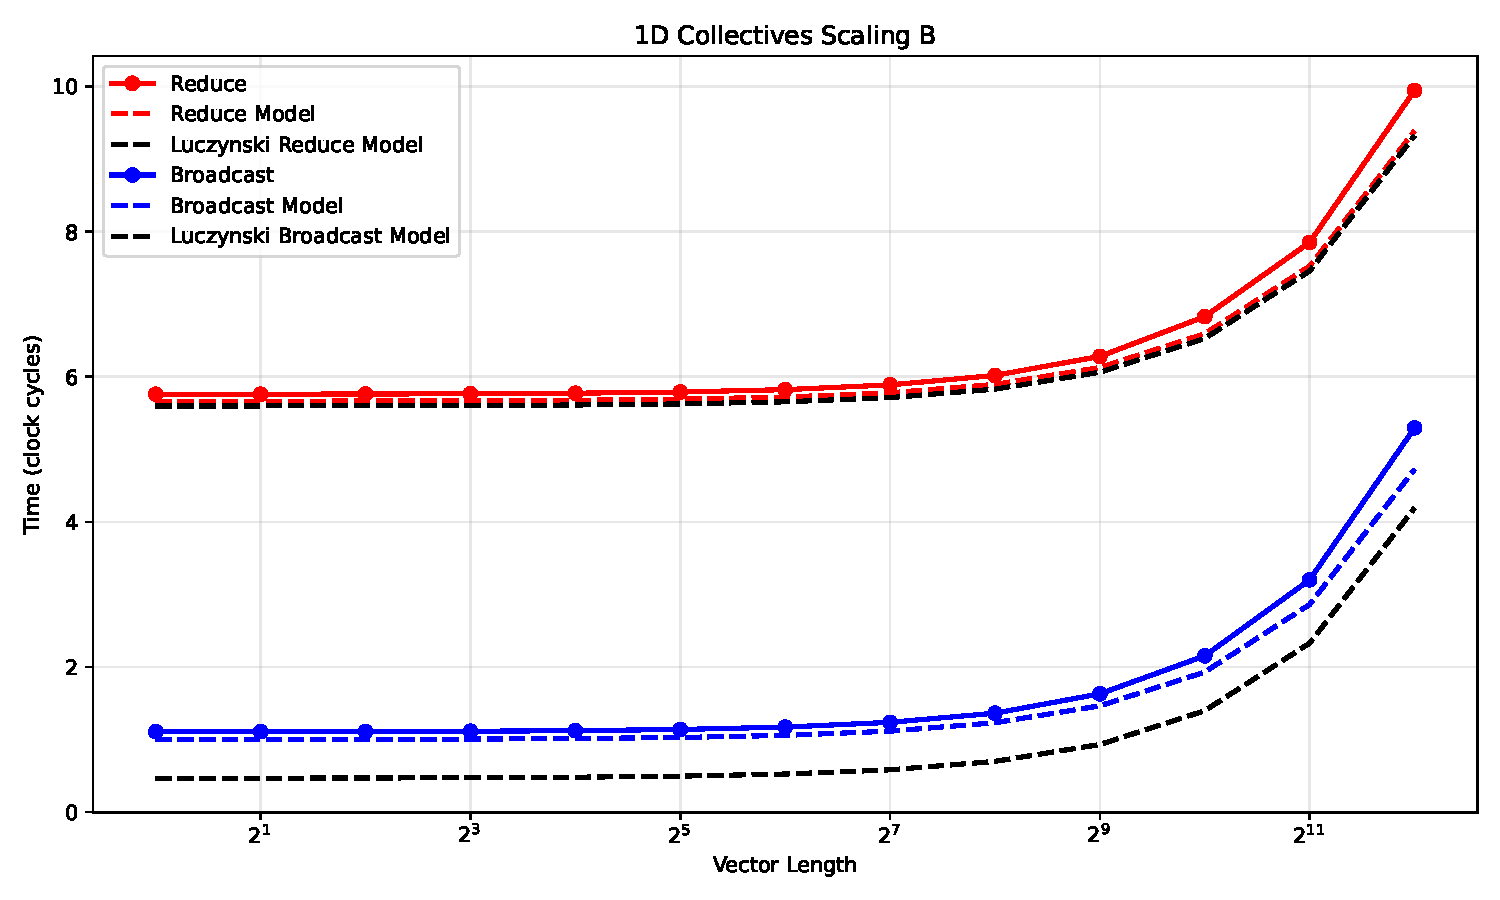
\includegraphics[width=\linewidth]{figures/collectives_scaleB.pdf}
        \caption{Evaluation of 1D collectives using a single row of 512 PEs.}
    \end{subfigure}
    \hfill
    \begin{subfigure}{0.48\textwidth}
        \centering
        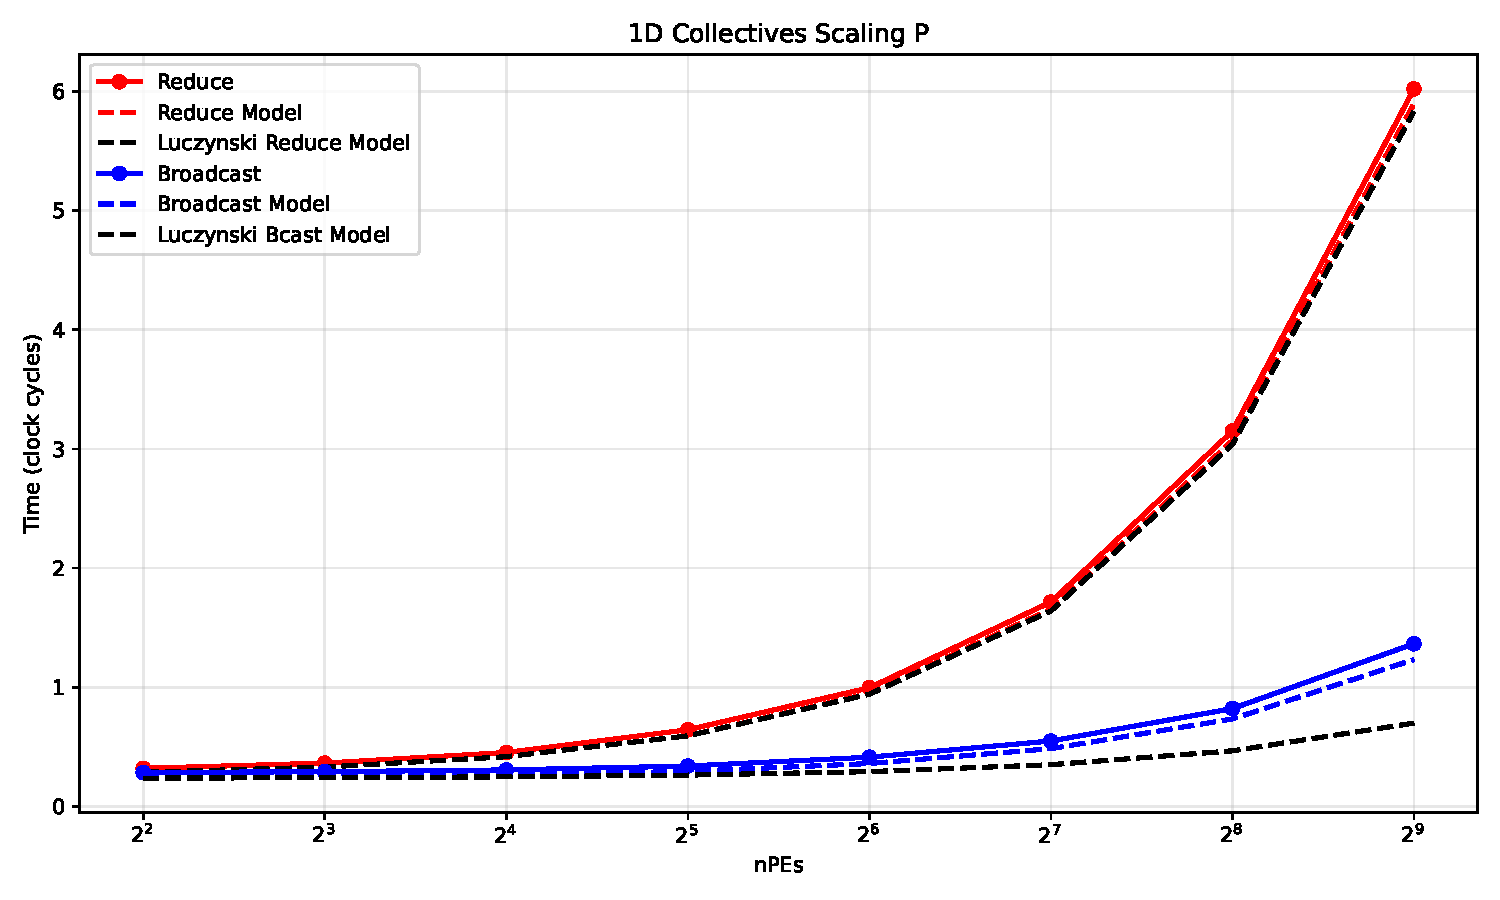
\includegraphics[width=\linewidth]{figures/collectives_scaleP.pdf}
        \caption{Evaluation of 1D collectives on vector of size 256 (1KB).}
    \end{subfigure}
    \caption{Main caption}
\end{figure}

\section{Two-Phase SpMV}
Solving $Ax = y$.
\begin{enumerate}
    \item The 1D collectives can be combined for SpMV.
    \item Distribute matrix nonzeros on the 2D mesh, Broadcast down rows, reduce across columns.
\end{enumerate}
\subsection{Sparse Partitionings}
\begin{enumerate}
    \item To use the 1D collectives, the matrix must be distributed in a row and column locality (RCL) fashion.
    \item My results explore a blocked, cyclic, and random partitioning of rows and columns.
    \item Load imbalance is important.
\end{enumerate}

\subsection{Dataflow Algorithm}
Assuming that the matrix $A$ is distributed on the 2D mesh under a mapping that preserves row and column locality, the SpMV can be conceptually
broken down into two simple 1D collective phases:
\begin{enumerate}
    \item Broadcast values of $x$ down mesh columns in the order prescribed by the mapping.
    \item Reduce rows of partial products across mesh rows also in the order prescribed by the mapping.
\end{enumerate}

Ensuring that broadcasts and reductions proceed in a prescribed order means that indices of $x$ and row indices of the reductions do not need to be communicated - instead, they are implied by the order of arrival.

In our implementation, the values of $x$ and the resulting values of $y$ are stored in 'moat' PEs: an extra row of PEs is set aside at the top of the
mesh onto which the initial values of $x$ are loaded. Similarly, an extra column of PEs is allocated to the left of the grid wherein the result values $y$ are stored
once computed.

Locally, each PE processes the SpMV in three distinct phases with serialization points between them.
\begin{enumerate}
    \item Store all incoming broadcasts for the PE column
    \item Complete all local compute for each output row
    \item Contribute all results to row reductions
\end{enumerate}
In theory, local synchronizations between these three components are not necessary. For example, early incoming broadcasts could trigger compute before all broadcasts are received.
While Tungsten does provide constructs that would support more overlap
of communication and computation here, we evaluated a couple different approaches and found that the serial approach consistently performed best.

Here it is important to note that while the kernel for each PE appears bulk-synchronous, the global algorithm is not. Broadcasts and reductions can proceed
as soon as the next individual PE is ready. In practice, this might look like reductions near the top of the grid completing before those lower in the grid.

\subsection{PE-Local Storage Format}
We implement two standard matrix storage formats: CSR and COO. These dictate only the storage of each PE's individual domain,
and therefore also the compute kernel per PE. Algorithm \ref{alg:csr} outlines the CSR algorithm, and Algorithm \ref{alg:coo} outlines the COO algorithm.
The COO format avoids the nested for loop and is therefore friendlier to the Tungsten compiler.
On the other hand, COO replaces the Aptr data structure, which has length corresponding to the number of local rows, with
a rowids data structure with an entry for each non-zero.

In evaluation in Section \ref{sec:coovscsr}, we find that COO is typically much more efficient than CSR.

\begin{algorithm}
    \caption{SpMV Kernel in CSR Format}
    \label{alg:csr}
    \begin{algorithmic}[1]
        \ForAll{$r \in \texttt{rows}$}
        \State $sum \gets 0$
        \For{$nnz \gets \texttt{Aptr}[r]$ \textbf{to} $(\texttt{Aptr}[r+1]-1)$}
        \State $sum \gets sum + \texttt{vals}[nnz] \cdot \texttt{x}[ \texttt{colids}[nnz]]$
        \EndFor
        \State $\texttt{partial}[r] \gets sum$
        \EndFor
    \end{algorithmic}
\end{algorithm}

\begin{algorithm}
    \caption{SpMV Kernel in COO Format}
    \label{alg:coo}
    \begin{algorithmic}[1]
        \ForAll{$n \in \texttt{nnzs}$}
        \State $sum \gets \texttt{vals}[nnz] \cdot \texttt{x} [\texttt{colids}[nnz]]$
        \State $r \gets \texttt{rowids}[nnz]$
        \State $\texttt{partial}[r] \gets \texttt{partial}[r] + sum$

        \EndFor
    \end{algorithmic}
\end{algorithm}

\section{Modeling SpMV}
\textcolor{red}{BIG IDEA 0. what is the performance model and what are its shortcomings}
\subsection{Communication}
\begin{enumerate}
    \item The 1D collectives model the communication of SpMV
    \item Whole SpMV communication can be approximated with just 1 reduction (correct P and B) and 1 broadcast. Think of this as matching the broadcast from top right down to bottom right, and then the reduction along the whole bottom row. This is the largest comm distance and the limiting factor.
    \item Vertical bcast requires small reticle adjustment because tehre are fewer reticle
\end{enumerate}

\subsection{Compute}
\begin{enumerate}
    \item record local compute time on every PE. Take the max.
    \item In practice, all compute does not happen perfectly in parallel. This is an approximate understanding of compute.
\end{enumerate}

\section{Experimental Setup}
We evaluate our SpMV algorithm and communication model on a WSE-3 in 32-bit floating point precision. The GPU baseline comparisons
are made with a cuSparse implementation evaluated on a single H200.
\subsection{Matrix Selection}
We evaluate on two classes of matrices: custom randomly generated matrices and a selection of matrices from SuiteSparse.
The randomly generated matrices are tunable based on matrix size and number of nonzeros. Nonzeros are placed uniformly at random.

A selection of SuiteSparse matrices is chosen for evaluation to capture SpMV performance on more real world use-cases
across a variety of applications, structures, and sizes. Our selection is outlined in Table \ref{tab:suite_sparse_matrices}.

\begin{table*}[t]
\centering
\caption{Suite Sparse matrices used in evaluation}
\label{tab:suite_sparse_matrices}
\begin{tabular}{lrrrl}
\toprule
name & id & nrows & nnz & category \\
\midrule
GHS\_psdef/crankseg\_1 & 1257 & 52804 & 10614210 & Structural Problem \\
Muite/Chebyshev4 & 1867 & 68121 & 5377761 & Structural Problem \\
DIMACS10/kron\_g500-logn17 & 2490 & 131072 & 10228360 & Undirected Multigraph \\
VLSI/radiation & 2839 & 223104 & 5526637 & Semiconductor Device Problem \\
SNAP/com-Youtube & 2783 & 1134890 & 5975248 & Undirected Graph With Communities \\
Dziekonski/dielFilterV2real & 2386 & 1157456 & 48538952 & Electromagnetics Problem \\
Bourchtein/atmosmodl & 2267 & 1489752 & 10319760 & Computational Fluid Dynamics Problem \\
LAW/indochina-2004 & 2451 & 7414866 & 194109311 & Directed Graph \\
DIMACS10/delaunay\_n23 & 2478 & 8388608 & 50331568 & Undirected Graph \\
VLSI/stokes & 2845 & 11449533 & 349321980 & Semiconductor Process Problem \\
SNAP/twitter7 & 2796 & 41652230 & 1468365182 & Directed Graph \\
MAWI/mawi\_201512020030 & 2802 & 68863315 & 143414960 & Undirected Weighted Graph \\
\bottomrule
\end{tabular}

\end{table*}


\subsection{WSE Pre-processing}
Once a matrix is chosen, a pre-processing step generates the corresponding input files for the WSE.
This step requires the matrix itself, the size of the PE grid, the mapping strategy (blocked, cyclic, random), and the format (COO, CSR).
The result of pre-processing is a set of binary files describing the data to be loaded on to the device.
This pre-processing step is not measured in algorithm runtime, and would in theory be reusable across multiple iterations of SpMV on the same matrix.

\section{Evaluation}

\subsection{COO vs CSR}
In all subsequent evaluation, we use COO.
\label{sec:coovscsr}
\begin{figure}[]
    \centering

    \begin{subfigure}{\linewidth}
        \centering
        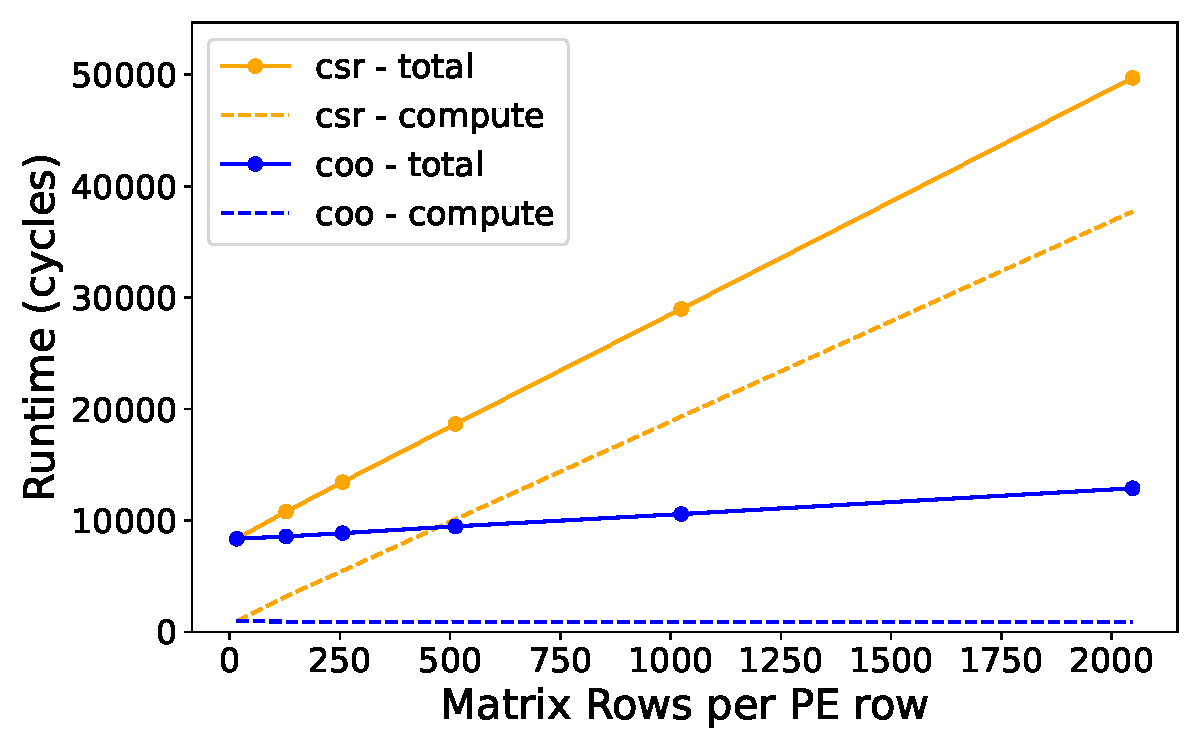
\includegraphics[width=\linewidth]{figures/compare-coo.pdf}
        \caption{Scaling rows.}
        \label{fig:compare-coo-scalerows}
    \end{subfigure}
    \hfill
    \begin{subfigure}{\linewidth}
        \centering
        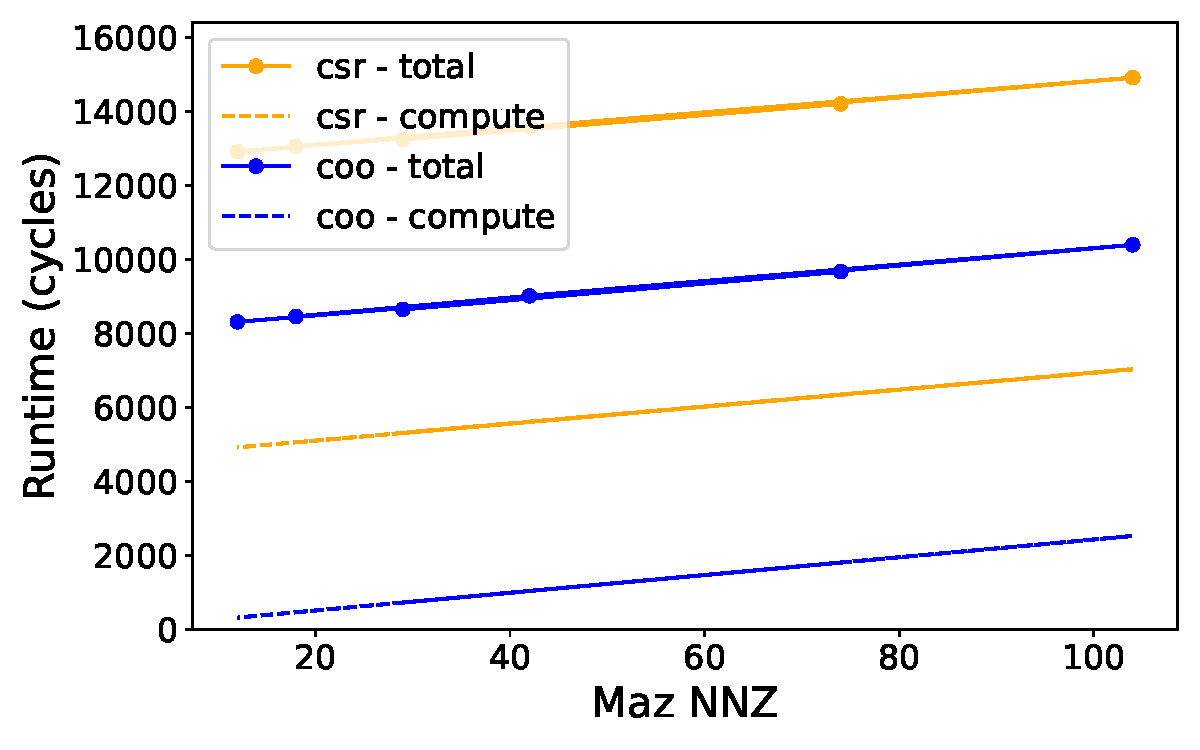
\includegraphics[width=\linewidth]{figures/compare-coo-scalennz.pdf}
        \caption{Scaling nonzeros.}
        \label{fig:compare-coo-scalennz}
    \end{subfigure}

    \caption{Comparison of the COO implementation under two scaling studies.}
    \label{fig:compare-coo}
\end{figure}

\subsection{Model Evaluation}
\textcolor{red}{BIG IDEA 1. is the performance model accurate}

Initial model evaluation is performed using randomly generated matrices.
The goal is to evaluate the accuracy of the performance model under the assumption of uniformly distributed nonzeros, and associated relative load balance.
Section \ref{sec:layout} will explore the impact of load imbalance and more realistic matrices.
these plots use the randomly generated matrices, no need to talk about load imbalance yet


\begin{figure}
    \centering
    \centering
    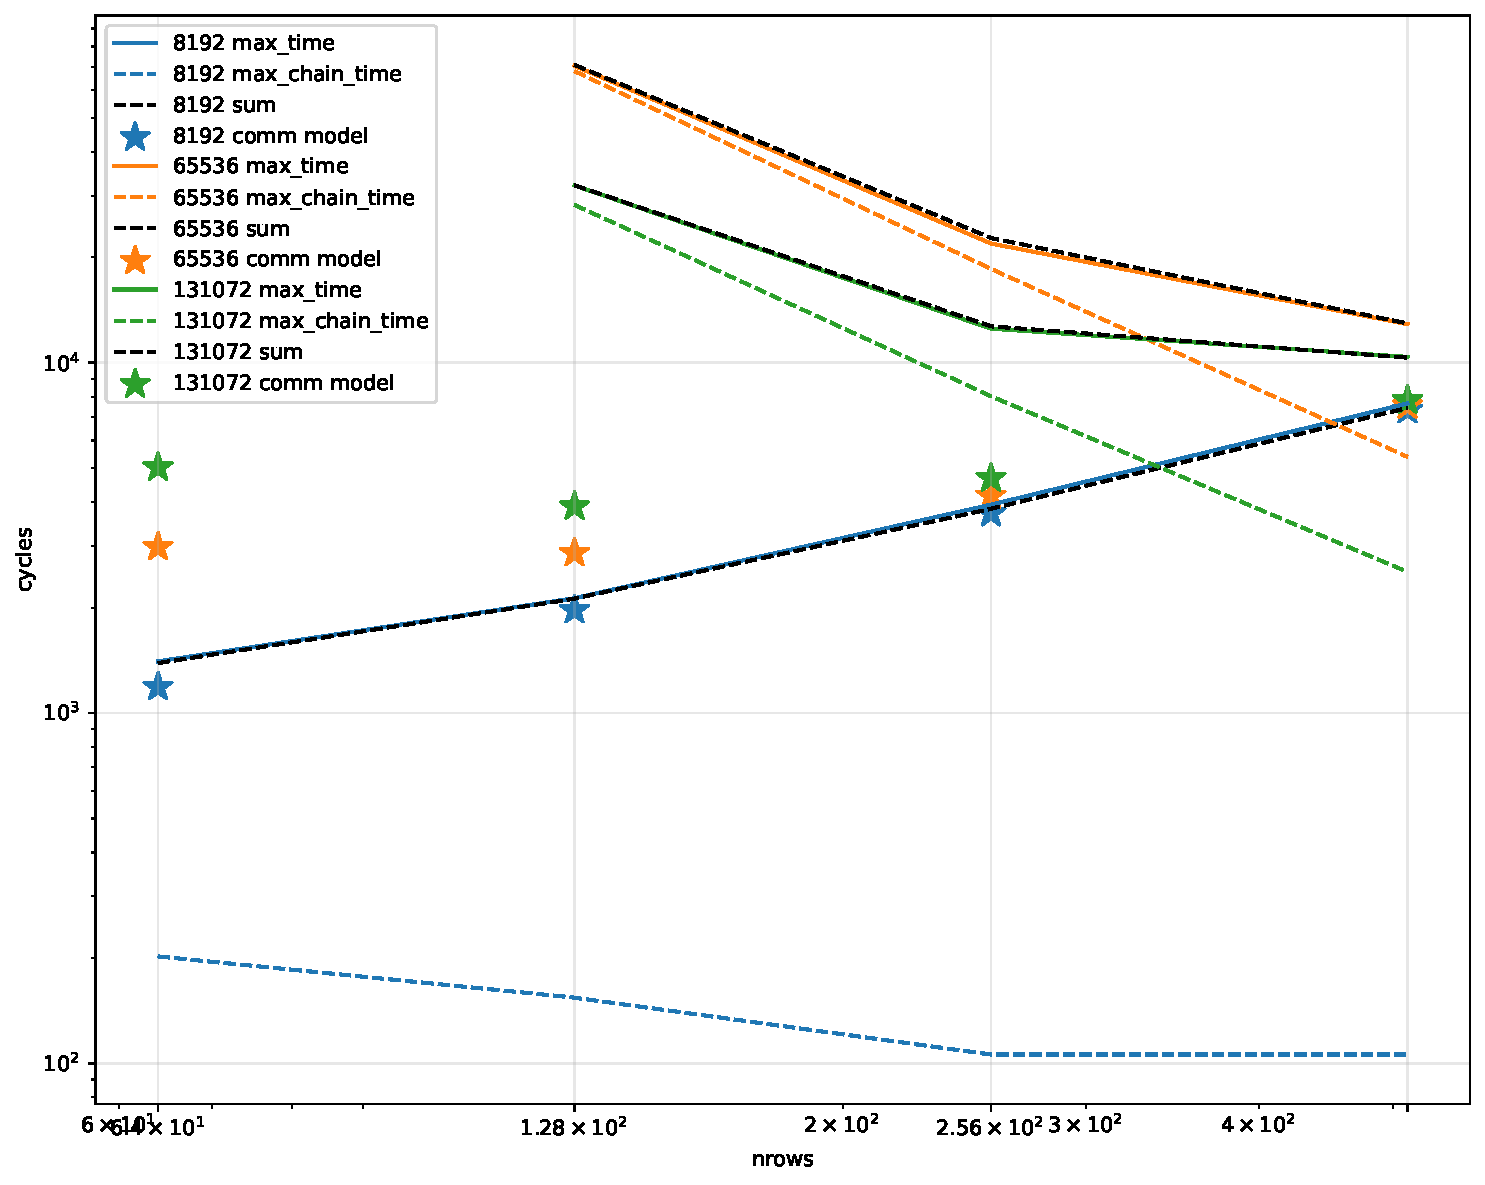
\includegraphics[width=\linewidth]{figures/random-scale-npes.pdf}
    \caption{PE Dim Scaling for 3 different matrices}

    \label{fig:scale-npes}
\end{figure}



\subsection{Matrix Layout}
\label{sec:layout}

Our selection of SuiteSparse matrices are an important addition to evaluation because they introduce structure which produces load imbalance, particularly under the basic 2D blocked decomposition. These matrices highlight
the utility of other mapping schemes.
Figure \ref{fig:suite-sparse-parameters} illustrates a first pass over the SuiteSparse selection under each of our three
mapping schemes, demonstrating how each scheme and matrix combination produces a different max nnz count.

This gives us a sense of how each mapping performs, based on the estimated maximum time spent in compute. The blocked
mapping typically introduces the most load imbalance, and cyclic and random often perform similarly.

The horizontal and vertical lines in Figure \ref{fig:suite-sparse-parameters} highlight the memory constraints of the WSE and the limitations
on the matrices and configurations our algorithm supports. The local 48KB limit per PE restricts both the number of nonzeros a PE can store and
the number of rows mapped to a single PE row (equivalently for columns). The horizontal line represents the nnz cap, and the vertical line represents the row count cap.
Note that these two caps are in fact dependent on eachtoher because the core PE mesh must store an array entry for each nonzero and an array entry for each local row. The lines don't reflect this dependency, but simply designate the apparent cutoffs not theoretical limits.

Of the 12 matrices in our random suite sparse selection, only 7 can be mapped to the hardware, and only under certain mapping schemes.





\begin{figure}
    \centering
    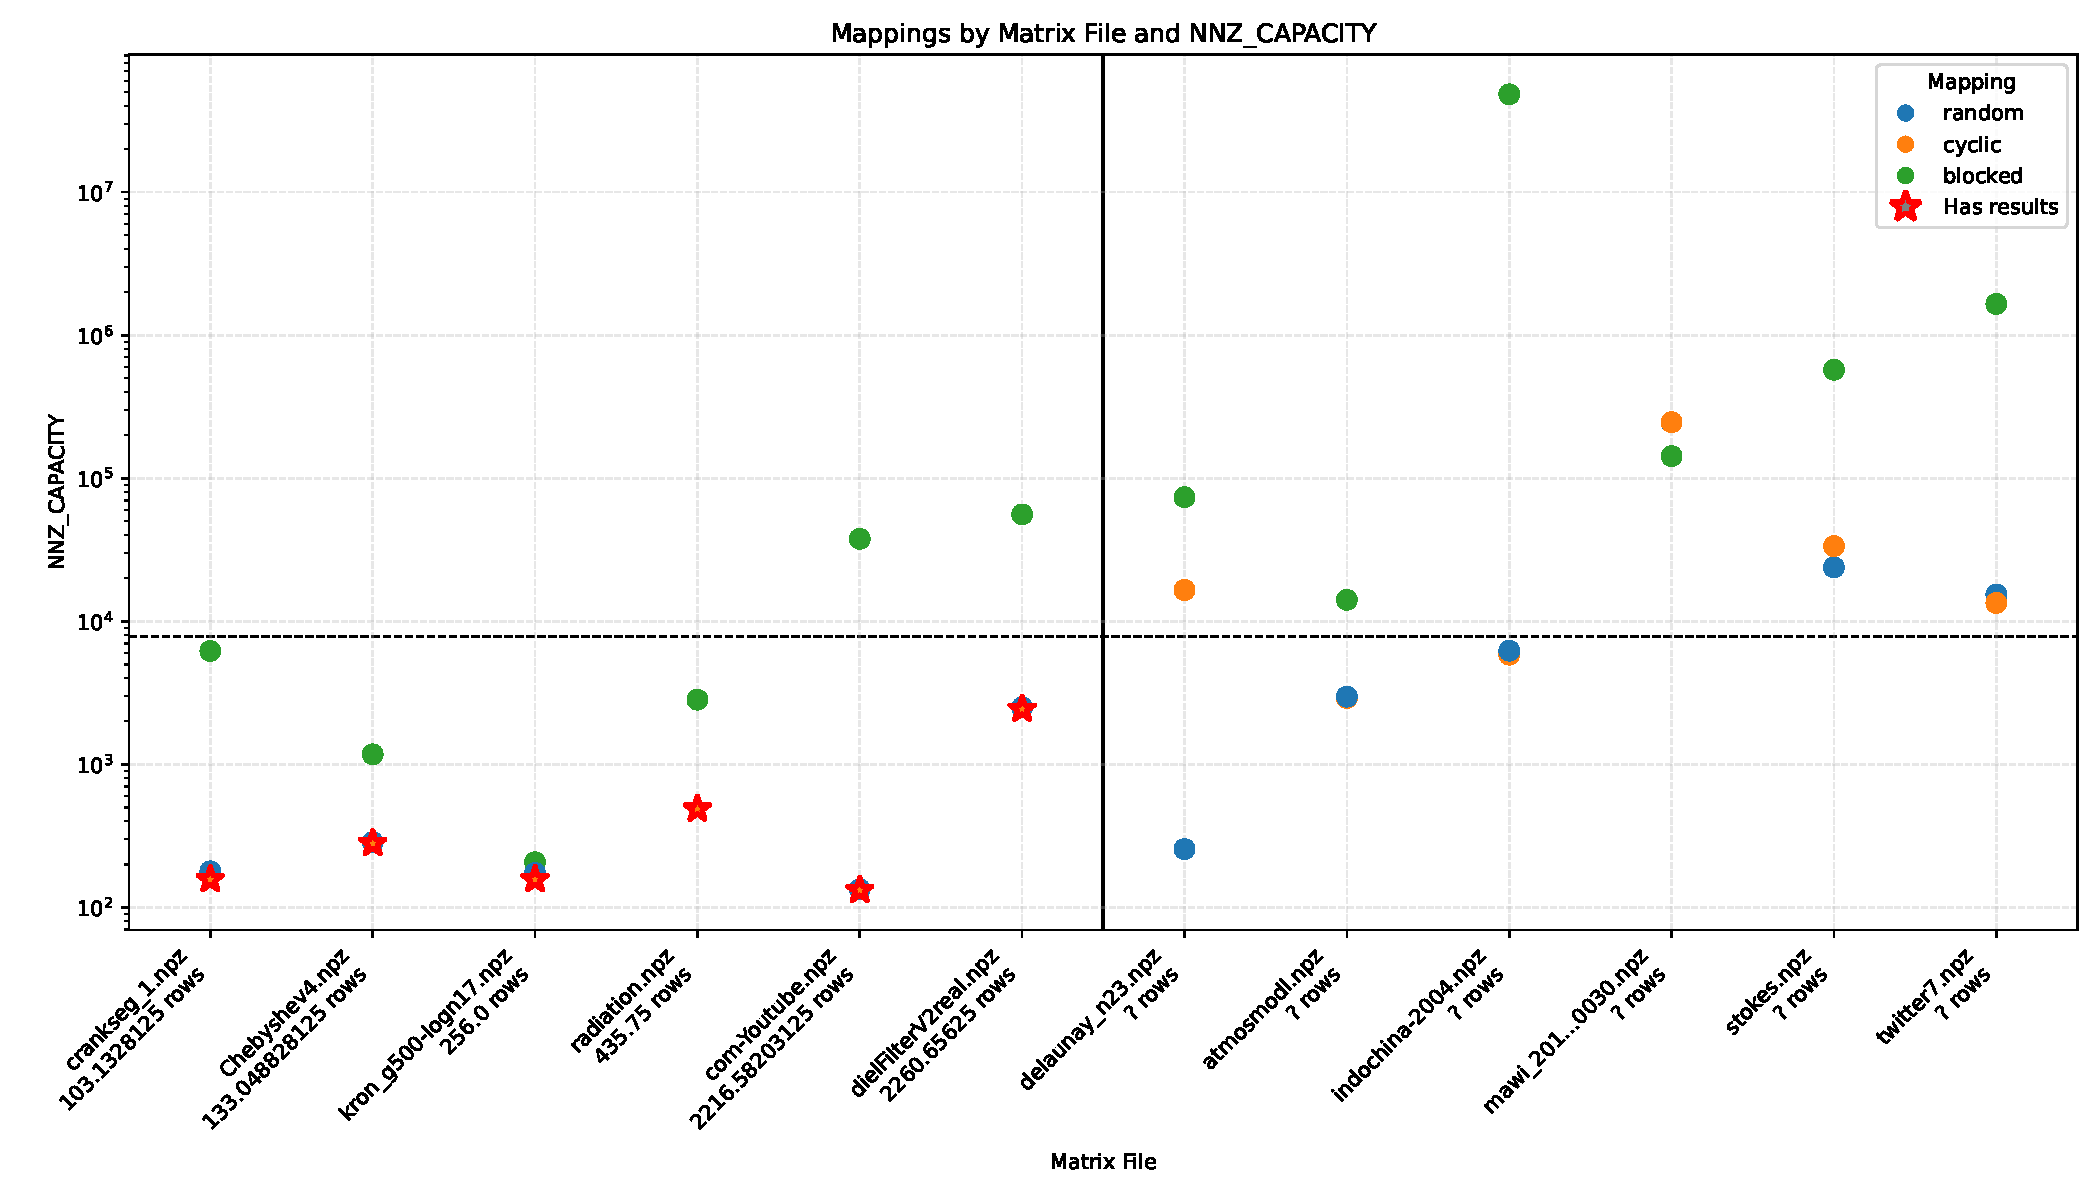
\includegraphics[width=\linewidth]{figures/suite_sparse_manifest.pdf}
    \caption{Parameter space evalutation of suite-sparse selection.}
    \label{fig:suite-sparse-parameters}
\end{figure}

\subsection{Configuration Selection}
\textcolor{red}{
    BIG IDEAS 2 and 3: how do we make decisions about layout and resources for optimal performance?
    lower and upper performance bounds for a given matrix/matrix type?
}

Not really sure if I can say anything here\dots

\subsection{SuiteSparse Breakdown}
Breakdown of performance by phase and by communication vs computation in Figure \ref{fig:suite-sparse-comm-model}
Note that the number of nnzs corresponds exactly to the compute time.
\begin{figure}
    \centering
    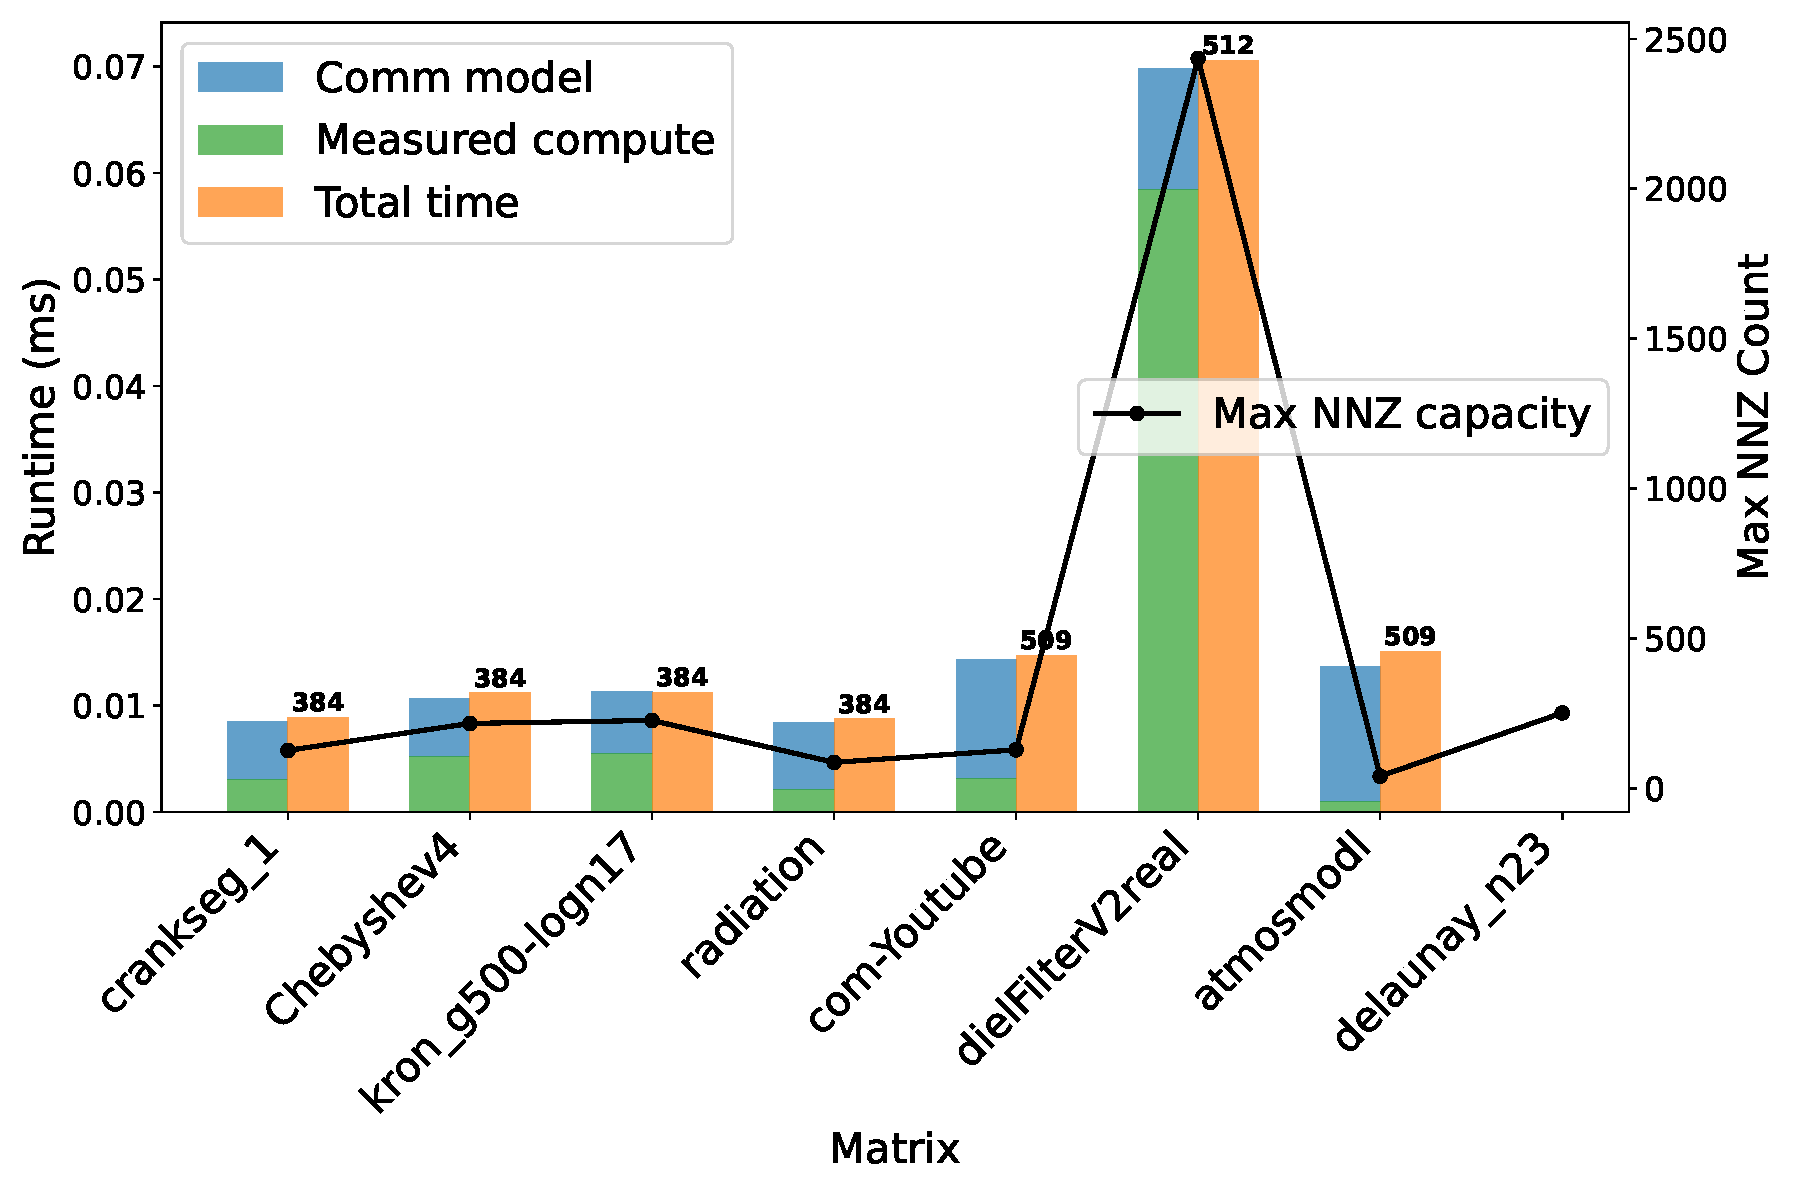
\includegraphics[width=\linewidth]{figures/suite_sparse_comm_model.pdf}
    \caption{Performance evaluation of SpMV with model breakdown on the WSE for various matrices from the SuiteSparse collection.}
    \label{fig:suite-sparse-comm-model}
\end{figure}


\subsection{GPU Comparison}
\textcolor{red}{BIG IDEA 4. is the spmv performant? and compare to GPU}

GPU comparison is a datapoint, not 'comparison'. Other factors like writing custom gpu kernels and power draw
use default cusparse CSR and collect all the cusparse configurations


1. the impact of structure (same number of nnz)
2. suite sparse performance
both runtime and throughput plots (maybe throughput put Triad throughput as comparison)

\textcolor{green}{TODO: the suite sparse matrices have substantially little nnz per row. do a scaling comparison with randomly generated matrices to look at larger nnz per row}, performance across randomly generate matrices


\begin{figure}
    \centering
    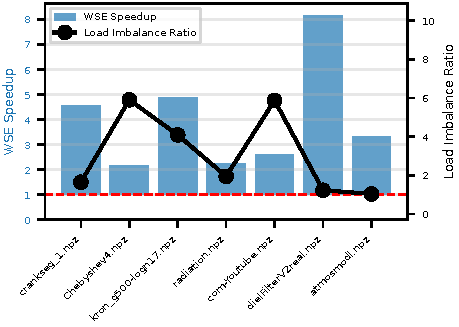
\includegraphics[width=\linewidth]{figures/suite_sparse_gpu_comparison.pdf}
    \caption{Speedup of WSE SpMV over GPU SpMV for various matrices from the SuiteSparse collection.}
    \label{fig:suite-sparse-gpu-comp}
\end{figure}



\section{Conclusion}

\bibliography{main}

\end{document}
